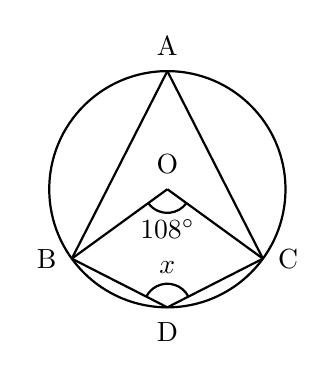
\begin{tikzpicture}[scale=1]

    % Define the center of the circle
    \coordinate (O) at (0,0);

    % Draw the circle
    \draw[thick] (O) circle (1.5);

    % Define points on the circle
    \coordinate (A) at (90:1.5);
    \coordinate (B) at (216:1.5);
    \coordinate (C) at (324:1.5);
    \coordinate (D) at (270:1.5);

    % Draw the lines and segments
    \draw[thick] (A) -- (B);
    \draw[thick] (A) -- (C);
    \draw[thick] (O) -- (B);
    \draw[thick] (O) -- (C);
    \draw[thick] (B) -- (D);
    \draw[thick] (C) -- (D);

    % Draw the angle arcs
    % Arc at O
    \draw[thick] (216:0.3) arc (216:324:0.3);
    
    % Arc at D (Fixed)
    % The line DC is at 27 degrees and DB is at 153 degrees relative to D
    \draw[thick] (D) ++(27:0.3) arc (27:153:0.3);

    % Add labels for the points
    \node[above, yshift=2pt] at (A) {A};
    \node[left, xshift=-2pt] at (B) {B};
    \node[right, xshift=2pt] at (C) {C};
    \node[above, yshift=2pt] at (O) {O};
    \node[below, yshift=-2pt] at (D) {D};

    % Add angle values
    \node at (270:0.5) {$108^{\circ}$};
    \node at (270:1.0) {$x$};

\end{tikzpicture}